%  \documentclass{sig-alternate}
%\documentclass[conference]{IEEEtran}
\documentclass{sig-alternate-05-2015}


\usepackage{cite}
\usepackage{url}
\usepackage{color}
\usepackage{tikz}
\usepackage{balance}
\usepackage{caption}

%%%%
\usepackage{pgfplotstable}
\usepackage{pgfplots}
\pgfplotsset{compat=newest}

\usepgfplotslibrary{statistics}
\makeatletter

\pgfplotsset{
  /pgfplots/flexible yticklabels from table/.code n args={3}{%
    \pgfplotstableread[#3]{#1}\coordinate@table
    \pgfplotstablegetcolumn{#2}\of{\coordinate@table}\to\pgfplots@yticklabels
    \let\pgfplots@yticklabel=\pgfplots@user@ticklabel@list@y
  }
}

\pgfplotsset{
   boxplot/every median/.append style={thick},
   boxplot/every average/.append style={thick},
   boxplot/every outlier/.append style={thick}
}

\usetikzlibrary{patterns} %% Bar chart

\newcommand{\todo}[1]{\textcolor{cyan}{\textbf{[#1]}}}
\newcommand{\mei}[1]{\textcolor{green}{{\it [Mei says: #1]}}}
\newcommand{\dan}[1]{\textcolor{blue}{{\it [Dan says: #1]}}}
\newcommand{\yasmine}[1]{\textcolor{red}{{\it [Yasmine says: #1]}}}


\begin{document}

\title{XXXXX}
% Does Marshmallow help users remember the permissions?
% How Does Marshmallow affect


\author{
%
% 1st. author\
\alignauthor
XXXXXX 	\\
%	\affaddr{Software Engineering Department}\\
       \affaddr{Rochester Institute of Technology, Rochester, NY, USA}\\
       \email{\{xxxx,xxxxx,xxxxx\}@rit.edu}
       \alignauthor
} % Must not be a space above this


%   ynevse
%   pkmvse


\maketitle
\begin{abstract}


% Introduce the problem that we are trying to solve
% How did I do my study
% What did I find?

Android applications (apps) rely on a permission-based model to carry out core functionality. The way that Android apps ask a user to accept permissions has recently changed from being an all or nothing accept or reject upon installation the application, to now asking for permission at runtime. A primary goal of this change was to provide users more control of the permissions their apps utilize. Do users actually feel more comfortable with this change? Are they more knowledgeable about the permissions their apps are using? 

We conducted a large, in person study involving more than 330 participants from a diverse background set to determine if this new permission model makes users feel more comfortable and knowledgable about the permissions their apps are using. We also sought to determine what impact providing a rationale had on user's accepting permission requests.

We found that.....


%%% Update abstract with what our paper actually explored.


\end{abstract}

%%% Are these good keywords???
\begin{keywords}

XXXXXX

\end{keywords}


\section{Introduction}
Android has become the world?s most popular mobile platform, allowing users to perform a variety of tasks that were previously unachievable in a mobile environment. Android applications (apps) provide the user with a diverse set of functionality allowing them to do everything from posting their Facebook status, to performing banking transactions. In order to perform various sensitive tasks, an app must be granted appropriate permissions to carry out this functionality. For example, if an app requests access to a user's contact list, the app much explicitly ask the user for permission to access this information. These app permissions serve as as an integral component of the app's security by limiting access to this information and functionality to other potentially malicious apps installed on the user's device, but also in ensuring that a user is adequately able to protect the information on their phone as they desire.

In Since its inception, Android has used a system where users were asked to accept all of an app's permissions at install time. If they did not approve all of an app's requested permissions, they would not be allowed to install or use the app. Numerous works stated issues with this design from numerous perspectives ranging from security issues since a user might not perform an important security update to an app since it requested a permission they did not approve of to more simple usability issues. \todo{cite} % Be specific, don't just say ``numerous''

The manner in which apps requested permissions substantially changed with the introduction of Android Marshmallow (Android M), which adopted a process of an app asking for permissions at runtime, and not install time. Users are now able to choose to provide an app specific functionality while still installing and using an app (without the functionality afforded by the permission), and even change the app's permission settings whenever they pleased, even long after installation.


%%% Probably add a few reasons for switching to M here
The conversion to this new permission structure had several intentions including making users feel more comfortable, streamline the app installation process, and provide them more authority over their data and privacy, and allow for automatic updates since a user would no longer be required to accept all changed permissions at install time\cite{android_developer_URL}.

% M = streamline app install process, provide more control over permissions & functionality. Revoke permissions at any time



We sought to determine if these goals were being met by performing a large study involving 321 participants from  diverse backgrounds. Our primary research questions were: \todo{add in RQs}

%% What are the current gaps


% Very clearly state the contributions of the paper


% The rest of the paper is organized as follows: In Section~\ref{sec:relatedworks}



%%% Primary Research questions

%   RQX: What effect does the new permission model have on a user's ability to recall an app's permissions?
%   RQX: What effect does the rationale have on a user's perception of a permission request?
%   RQX: Which model helps users feel more Comfortable?




%%% Secondary
%   Well well are users able to identify


\section{Background \& Related Work}
\label{sec:relatedworks}

% https://pure.strath.ac.uk/portal/files/44777319/Robinson_Weir_ICGS2015_understanding_android_security.pdf



%%% Add more to this depending on the conference we submit to

\subsection{Android Permissions}


Android apps operate under a privilege-separated system where each app operates with a specific system identify, and each app is isolated from all other apps on the device. More fine-grain functionally enforces permissions on specific operations which the app may carry out. For example, if an app wishes to access the internet, or the user's contacts, the app will be required to be granted this permission before the app has the ability to access this functionality. Permissions are separated into several protection levels, with the most important being \emph{normal} and \emph{dangerous} permissions~\cite{android_permissions_URL}. 



\begin{enumerate}
 \setlength{\itemsep}{.8pt} 
    \setlength{\parskip}{0pt} 
    \setlength{\parsep}{0pt}  


	\item \textbf{Normal}: These permissions cover functionality that the app needs which are located outside of its sandbox, but are deemed to create very little risk to the user's privacy, or to other apps. An app that requests a normal permissions is automatically granted this functionality. In Android Marshmallow, some normal permissions include \texttt{BLUETOOTH},\texttt{ACCESS\_WIFI\_STATE} and \texttt{INTERNET}. 
	\item \textbf{Dangerous}:  These permissions are deemed to pose significant risks to the user's privacy, or to other apps installed on the device. The user must explicitly grant access to any dangerous permissions requested by the app.  In Android Marshmallow, some dangerous permissions include \texttt{READ\_CALENDAR}, \texttt{READ\_SMS} and \texttt{CAMERA}. In Android Marshmallow, all dangerous permissions belong to a specific permission group. For example, all dangerous permissions which are related to phone calls belong to the \emph{Phone} group. When an app requests a dangerous permission in a group which the user has already granted a permission in, the app automatically gains the ability to use that permission since the app has already been granted a permission in that group. For example, if the app requests the \texttt{CALL\_PHONE} permission, but the app has already been granted the \texttt{ADD\_VOICEMAIL} permission, the app will automatically gain access to the \texttt{CALL\_PHONE} permission since they both reside in the same group.

\end{enumerate}

Prior to Android Marshmallow, the user was prompted to accept or reject all dangerous app permissions whenever installing an app. When updating an app, they were also prompted to accept or reject all new permissions the app was requesting. If the user desired to not approve even a single permission, they would not be allowed to update install the app. It was an all other nothing ordeal. Users were also not able to change permissions after installation and the only way to restrict an app's access to a specific permission was to uninstall the entire app~\cite{Wijesekera:2015:APR:2831143.2831175}. In the past several years, there has been a substantial amount of research recommending changes to the Android permission model ranging from the creation of privacy profiles~\cite{Liu:2014:RMA:2566486.2568035} to more granular sets of Android permissions~\cite{7145666}.

Marshmallow represented a significant change with how permissions were handled in Android apps. Users would now be prompted about allowing an app's permission requests at runtime, and not upon installing the application. The intention is that this would make installing and updating the app a simpler, easier process while providing the user greater access over the app, and therefore their privacy. The user would also be able to use the app, but choose the permissions they wanted to allow it to have, and even change their permission decisions whenever they pleased. The developer would also have the option of providing a \emph{rationale}, or further explanation, to the user about why the app was asking for a particular permission.


%-- General info
%\cite{biswas2016android} %%% Probably not alll that useufl



\subsection{Related Work}


%   The first examining the M model
%   List all the papers which called for changes in the M structure
%   How were other user studies carried out (such as the felt study)

% Felt:2012:APU:2335356.2335360

\section{Methodology} % User Study
\label{sec: method}

-- Introduce user study \& hypothesis


% Mention the number of users and then talk about things like how many users were removed for being under 18
% 


\subsection{Hypothesis}

Upon beginning our work, we began with several hypothesis:


\begin{enumerate}
 \setlength{\itemsep}{.8pt} 
    \setlength{\parskip}{0pt} 
    \setlength{\parsep}{0pt}  


%%% Provide more citations and reasons why we believe this

	\item \textbf{Marshmallow helps users feel more comfortable using the apps}:  The new permission model affords users greater control to choose the permissions that their app uses. We believe that this will make users feel more comfortable with using the apps.
	\item \textbf{ Permissions in Android M are easier to understand and recall if we add meaningful rationale to the requested permissions}:  (find external works to back this up or support it) - \todo{Find reasons to back up the way I believe that I do}
	\item \textbf{Most users still have poor comprehension of Android permissions}:  Previous research has also shown that the majority of users do not properly comprehend what permissions actually mean ~\cite{Felt:2012:APU:2335356.2335360}. We believe that our findings for both the Pre-M and Marshmallow versions of the app will support these previous findings. \todo{add more citations}
	\item \textbf{Providing a rationale will help users feel more comfortable with accepting permissions}:  XXXXX\todo{find rationale}
	\item \textbf{Most users will continue to pay little attention to permissions}:  Previous research conducted on the Pre-M permission model has shown that most users do not pay attention to permissions when installing an app~\cite{Felt:2012:APU:2335356.2335360}. Although the new Marshmallow model will provide users with more control, and in many ways make them more aware of the permissions they are installing, we still believe that permission attention will continue to be a problem.
%	\item \textbf{Danz}: 
%	\item \textbf{Danz}: 
%	\item \textbf{Danz}: 

\end{enumerate}




%%% Make sure to find other works to back up my hypothesis


\subsection{Study Design}

%% Mention the primary components of our study
Our study was comprised of three primary components: User Recruitment, the Tic-Tac-Toe app, and Questionnaire, which we will describe.

\subsubsection{Recruitment}

Our human study was conducted at Imagine RIT\footnote{\url{http://www.rit.edu/imagine/}}, a single day event where thousands of members of the community visit the RIT campus and view a variety of scientific and educational venues ranging from robotics, software projects, and engineering activities. With the assistance of student volunteers, we set up two tables with six MacBook laptops running an Android emulator. Two laptops were running the emulator with API 22 (Pre-M), while the other four were running API 23 (Marshmallow). Participants were recruited by asking visitors passing by our table if they would like to participate in an Android study. Users were only provided vague details about the study being about Android permissions in the event pamphlet.

\subsubsection{Application}

We developed a simple tic, tac, toe app for use in our study, which contained the following permissions: \texttt{ACCESS\_FINE\_LOCATION}, \texttt{GET\_ACCOUNTS} and \texttt{READ\_PHONE\_STATE}. We selected these permissions since they have been identified as commonly used permissions in Ad libraries~\cite{liu2015efficient}.  When beginning to use the app, users were told to act like they were using the app on their personal device and were randomly asked to participant using one of three nearly identical versions of the app:

\begin{enumerate}

    \item  \textbf{Android Pre-Marshmallow} (API 22): Users were asked to accept or deny all app permissions at install time, a process which replicates how Android has asked users for permissions since its inception.

    \item  \textbf{Android Marshmallow - No Rationale} Users were asked to accept or reject permissions at runtime. At the beginning of the game, participants were told that the app needed to locate people around them and the user was asked if they wanted to allow the app to access the device's location. After playing the game, the app asked for the permissions to make calls and access the user's contacts.

    \item  \textbf{Android Marshmallow - With Rationale} (API 23): This version of the app was identical to the No Rationale version, except that a rationale was provided to the user before being prompted for their permission. For example, before asking for permission to access the user's contacts, a rationale stated that ``This App needs to access your contacts to share results.''

\end{enumerate}

Both Marshmallow versions of the app were connected to a database which recorded whenever a user accepted or denied a permission. Since all permission requests are made at installation for Pre-M apps, there was no data to record for this API level.

The app began by asking users to start a new game, and was followed by participants selecting several area participants to play against. Since the primary objective of the research was to understand how users react to the new permission model, we felt comfortable mocking out this functionality in the app. The participants would then play the game and were notified of their victory or defeat at the conclusion of the game. Once the game was completed, users were asked to share their results with the contacts on their device. 

\subsubsection{Questionnaire \& Exit Survey}

Before using the app, participants were initially asked to provide basic information about themselves such as age, gender, highest level of education, and how long they have used Android. Participants were not required to have ever used Android. After playing the game, participants were then asked to fill out the second portion of the questionnaire, which was nearly identical for all three of the user groups, except for certain questions pertaining to each group such as how helpful the permission rationale was, or if the user felt comfortable with accepting or rejecting permissions at runtime. Users were not allowed to go back and use the game to assist them in answering any of the questions, and were told to do the best they could in accurately answering all questions.

\section{Results}



Our work was driven by XXX primary research questions:\\

\textbf{RQX: What effect does the new permission model have on a user's ability to recall an app's permissions?}


\todo{find citations about why it is important for users to know the permissions in their app}

%% 


% Give more of an introduction as to what we did

A primary goal of the new permission model was for users to be more knowledgable about the permissions their apps were using. As part of our user study, we asked users how easy it was to recall the permissions they accepted and rejected


\todo{Pradeep: Get the numbers for this} %% Pradeep: Let's provide the statistics for the following questions and show them in the way that you feel is the most appropriate: 

%	How easy was it to recall what permissions you accepted?
%	How easy was it to recall what permissions you rejected?

\begin{figure}[!htb]
  \centering
  \begin{tikzpicture}
    %\tikzstyle{every node}=[font=\small]
    \begin{axis}[
	y=0.6cm,
	ytick={1,2,3},
	yticklabel style={align=center},
	yticklabels={Pre-M,M--No rationale,M--Rationale},
	width=6cm,
	xtick={1,2,3,4,5,6,7},
	xlabel={Ease of remembering permissions accepted},
	xlabel style={align=center},
	boxplot/average=auto,
	%title style={align=center},
	%title={Permissions accepted},
	%title style={yshift=-1ex,},
        %cycle list name=colorbrewer-RYB3,
	]
	\addplot+[boxplot]
	table[x expr=\coordindex, y index=0, col sep=comma]
	{ease-recall.csv};

	\addplot+[boxplot]
	table[x expr=\coordindex, y index=1, col sep=comma]
	{ease-recall.csv};

	\addplot+[boxplot]
	table[x expr=\coordindex, y index=2, col sep=comma]
	{ease-recall.csv};
    \end{axis}
  \end{tikzpicture}
  
  \vspace{1em}
  \begin{tikzpicture}
    %\tikzstyle{every node}=[font=\small]
    \begin{axis}[
	y=0.6cm,
	ytick={1,2,3},
	yticklabel style={align=center},
	yticklabels={Pre-M,M--No rationale,M--Rationale},
	%ytick=\empty,
	width=6cm,
	xtick={1,2,3,4,5,6,7},
	xlabel={Ease of remembering permissions rejected},
	xlabel style={align=center},
	boxplot/average=auto,
	%title style={align=center},
	%title={Permissions rejected},
	%title style={yshift=-1ex,},
        %cycle list name=colorbrewer-RYB3,
	]
	\addplot+[mark=x,boxplot]
	table[x expr=\coordindex, y index=3, col sep=comma]
	{ease-recall.csv};

	\addplot+[mark=x,boxplot]
	table[x expr=\coordindex, y index=4, col sep=comma]
	{ease-recall.csv};

	\addplot+[mark=x,boxplot]
	table[x expr=\coordindex, y index=5, col sep=comma]
	{ease-recall.csv};
    \end{axis}
  \end{tikzpicture}
  %\vspace{-2ex}
  \caption{Ease with which participants remember the permissions they
  accepted and rejected.}
  \label{fig:personality-strategy-novelty}
\end{figure}


We next sought to determine if users were actually able to recall the
permissions the app requested. As part of our post activity survey, we
asked to users to select all the permissions the app used from a list
of six possible options. We then measured the precision, recall and
F-score of the user's ability to correctly recall the permissions the
app had used. The results of this analysis are shown in
Figure~\ref{fig:remember}.


%%%% Make into a bar chart?
%\begin{table}[h]
%\begin{center}
%\caption{Ability to Recall App Permissions\todo{Find better way to describe this}} %%% Change the title
%\label{table:recallAppPermissions}
%\begin{tabular}{l|l|l|l}
%
%
%    \bfseries App Group & \bfseries Precision & \bfseries Recall & \bfseries  Accuracy \\ \hline\hline
%
%    \bfseries Pre-M & .71 & .43 & .62 \\ \hline\hline
%    \bfseries M - Rationale & .90 & .67 & .76 \\ \hline
%    \bfseries M - No Rationale & .90 & .64 & .74 \\
%
%\end{tabular}
%
%\end{center}
%
%\end{table}

\begin{figure}[!htb]
\centering
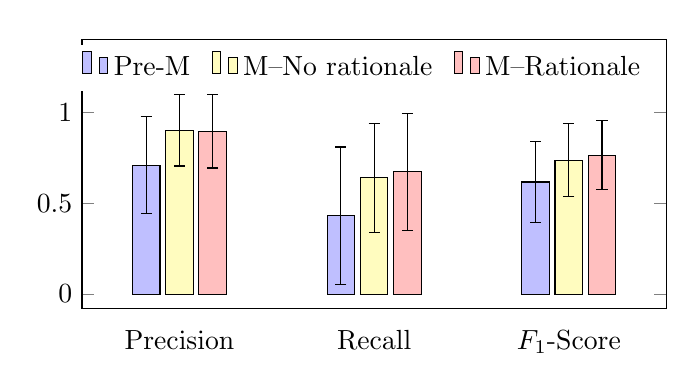
\begin{tikzpicture}
\begin{axis}[ybar,
    width=9cm,
    height=5cm,
    xtick={1,2,3},
    xticklabels={Precision, Recall, $F_1$-Score},
		enlarge x limits=0.25,
		xtick style={draw=none},
		ymax=1.4,
		legend style={draw=none,legend columns=-1,
		  /tikz/every even column/.append style={column sep=0.2cm}},
    ]

\addplot[
    fill=blue!25,
    draw=black,
    point meta=y,
    error bars/.cd,
        y dir=both,
        y explicit
] 
table [y error=error] {
x y error
1 0.7091 0.2652
2 0.4316 0.3772 
3 0.6164 0.2211 
};

\addplot[
    fill=yellow!25,
    draw=black,
    point meta=y,
    error bars/.cd,
        y dir=both,
        y explicit
] 
table [y error=error] {
x y error
1 0.9009 0.1967
2 0.6394 0.3
3 0.7360 0.2013
};

\addplot[
    fill=red!25,
    draw=black,
    point meta=y,
    error bars/.cd,
        y dir=both,
        y explicit
] 
table [y error=error] {
x y error
1 0.8958 0.2026 
2 0.6731 0.3217
3 0.7636 0.1904
};
\legend{Pre-M,M--No rationale,M--Rationale};
\end{axis}
\end{tikzpicture}
\caption{Participants' ability to remember permissions.}
\label{fig:remember}
\end{figure}


There was only a very small difference in the results between the `M - With Rationale' and `M - Without Rationale' groups, which is not surprising since the same permission requests were still shown at the same time to the users, with only an extra reasoning dialog shown to the with rationale group. However, there was a large difference in the three evaluated groups between the two `M' groups, and the `Pre-M' group. This demonstrates that users were able to more accurately able to recall the proper requested permissions for each of the Marshmallow groups in comparison to the Pre-M group. With the Pre-M model, users are shown the app's permissions at install time. Very frequently, users would quickly skim through this list in an attempt to use the app as soon as possible. Users also voiced their displeasure with the permission model in their feedback, with one user stating: ``Either you accept the condition of permission or you cannot install the application. that's a really annoying thing. I'd like to know why a particular app needs the permissions it needs.'' This lack of attention to the permissions in the Pre-M model is supported by previous research which demonstrates that few users pay attention to permissions when installing an app and that very few users are able to correctly recall the permissions an app uses~\cite{Felt:2012:APU:2335356.2335360}.




This demonstrates that % State the importance of these results







\todo{See if there is a correlation between the ability to recall permissions and if users said it was easy - Do on an individual level}


\textbf{Discussion:}
% Talk about ramifications/implications here. What is the "so what" ?

%	The new model does help users understand permissions better
%	Developers may want to switch to supporting the new model
%	Encourage end users to swtich (maybe talk about the fragmentation of Android and how updating is hard)




\textbf{RQX:} What effect does the rationale have on a user's perception of a permission request?


We next sought to determine the effect that providing a meaningful rationale had on a user accepting or denying a permission request. In order to explore this question, we provided users with nearly two identical versions of the same app, with the only difference being that one version provided users with a meaningful rationale as to why the permission was required. Whenever a user accepted or rejected a permission request, we recorded these results in a remote database. In the `With Rationale' version of the app, we provided a meaningful rationale as to why the app was requesting the permission before asking the user for their location (\texttt{ACCESS\_FINE\_LOCATION}) and if the app could have access to the contacts information on the device (\texttt{GET\_ACCOUNTS}). In order to act as a control between the two groups, we provided no rationale for the \texttt{READ\_PHONE\_STATE} permission. \dan{best way to say this?} The results of this analysis are shown in Table~\ref{table:permAcceptance}.

%Using the~\emph{shouldShowRequestPermissionRationale()} function, each user

\begin{table}[h]
\begin{center}
\caption{Permission Model User Acceptance} %%% Change the title
\label{table:permAcceptance}
\begin{tabular}{l|l|l}


    \bfseries Permission & \bfseries Rat Accept  & \bfseries No RatAccept  \\ \hline\hline
    \bfseries ACCESS\_FINE\_LOCATION & 0.95	 &	0.86  \\ \hline
    \bfseries GET\_ACCOUNTS & 0.62 &	0.49  \\ \hline
    \bfseries READ\_PHONE\_STATE & 0.59  &	0.57  \\ %\hline    			


\end{tabular}

\end{center}

\end{table}


%%% Does this rationale help users to feel more comfortable?

 These results demonstrate how a meaningful rationale can influence a person to accept



 Although we have found meaningful results, we believe that there is substantial room for future research in this area. For example, \todo{talk about the future work}


%% Discuss these results a bit


%% Demonstrates the need for future work in this area

 %  How the rationale






%%%% What is the takeaway messsage for developer's



\textbf{Discussion:}
% Talk about ramifications here.  What implications arise from this

%	Developers should use rationale
%	




\textbf{RQX:} Which model helps users feel more Comfortable?










%%% Further explore some of the statistics here

%      How many got the other permission questions correct
%      What do the general survey results say





%%%% So What

%   Developers should switch over to the new model
%   Demonstrates that the new model is effective
%

\section{Other Observations}
\label{sec:miss}



%   How many users could correctly answer questions about location, phone calls, accounts
%           Link into other works which say that users don't know much about privs
%   Do demographics/time of Android use play a role in things?
%   What were some general user preferences about how they felt? 



\section{Limitations \& Future Work}
\label{sec:futurework}

%% Did not have users use Marshmallow for extended periods of time, meaning that they did not use many of the other features such as altering permissions after installation or viewing all the apps that use a particular permission in the app menu

% Performed study only on laptop. Did not use actual Android device
% Do a longer, lab study like was done with Felt

\section{Conclusion}
\label{sec: conclusion}



\section*{Acknowledgment}

We would like to thank the following students for their contributions to the project: Hussein Talib, Cesar Fernandez, Silva Matti, Paula Garcia, Chris Lentner, Daniel Santoro, Taylor Corrello, Jodie Miu, George Hearde, and Kocsen Chung. This work was partially funded through a development grant from RIT



\balance % enable this
\bibliographystyle{abbrv}
\bibliography{MPermissions}

% That's all folks!
\end{document}


% ************************



%% Primary Research Questions
%	Do users recall M permissions more?
%	Does rationale help users feel more comfortable?
%	Do Android users actually understand permissions better than non-users?
%	


%%% Todo
%




%%% Venues
%	IEEE Software:



%	EMSE?



%%% Further work
%   Have rationales hide totally unnecessary permissions which could create privacy concerns
%   How can the rationale be worded to have users accept it?
%   Crowdsource the rationale






